\chapter{Infrastruktura kontinuiranog razvoja aplikacija}
Za izradu sustava za kontinuiran razvoj aplikacije potrebna je infrastruktura koja to omogućuje.
Postoji velik izbor aplikacija i servisa, koji se mogu koristiti za kontinuiran razvoj aplikacije.
Na primjer, za verzioniranje koda može se koristiti Git, Subversion, Mercurial, Microsoft TFS, a za
kontinuiranu integraciju programskog koda Jenkins, Hudson, TeamCity.

\section{Git - sustav kontrole verzija}
Sustav kontrole verzija je sustav koji sprema promjene datoteka kroz vrijeme. Najčešće se koristi za
pohranjivanje programskog koda, no takav sustav može se koristiti i za druge stvari kao što su
pisanje knjige, dokumenata, dizajn i slično.

Prilikom izgradnje programske podrške u pravilu je potrebno imati sustav verzija, pogotovo ako više
inženjera radi na istom projektu. Korisnik u bilo kojem trenutku može zapisati trenutno stanje mape
(\textit{engl.~directory}) u sustav. Na primjer, korisnik može zapisati kad je određena cjelina
aplikacija isprogramirana, kada je popravljena greška (\textit{engl.~bug}) ili kada su dodani novi
testovi jedinica. Korisnik može pregledati povijest u bilo kojem trenutku, vratiti mapu u prijašnje
stanje, usporediti izmjene između zapisa. To je samo mali dio operacija koje korisnik može odraditi.

\subsection{Vrste sustava kontrole verzija}
Prije nego što su ovakvi sustavi postali popularni i industrijski standard, korisnici su ručno
kopirali mapu ili datoteku te ju spremili kao rezervu (\textit{engl.~backup}). Takav proces podložan
je greškama te ne pruža puno funkcionalnosti. Jedno od prvih rješenja bio je RCS (\textit{engl.
Revision Control System})~\citep{chacon2014pro}, koji omogućuje pohranjivanje razlike datoteka
(\textit{engl.~patch set}) između revizija. Korisnik može vratiti datoteku u prijašnje stanje tako
da sustav primjeni razliku datoteka, kao što je prikazano na slici~\ref{fig:02rcs}.

\begin{figure}[h]
    \centering
    \begin{tikzpicture}[
        scale=0.7,
        start chain=1 going below,
        start chain=2 going right,
        node distance=6mm,
        text centered,
        box/.style={
            rectangle,
            rounded corners,
            draw=black,
            very thick,
            minimum height=12mm,
            fill=yellow!10
        },
        version/.style={
            fill=blue!10
        },
        l1/.style={
            text width=8cm,
            on chain=1,
            scale=0.9,
        },
        l2/.style={
            text width=8cm,
            on chain=2,
            scale=0.9,
        },
    ]

        \node [text width=8cm] (e1) {};
        \node [text width=8cm, right=of e1] (e2) {};
        % Lijevo
        \node [l1, below=of e1] (fs) {Datotečni sustav};
        \node [l1, minimum height=12mm] (empty) {};
        \node [box, l1] (file) {Datoteka};

        % Desno
        \chainin (fs); % Start right of file
        \node [l2] (rcs) {RCS - Revision Control System};
        \chainin (empty); % Start right of file
        \node [box, version, l2] (version3) {Verzija 3};
        \node [box, version, l2, continue chain=going below] (version2) {Verzija 2};
        \node [box, version, l2] (version1) {Verzija 1};

        \draw[<-] (file.east) -- (version2.west);
        \draw[<-] (version3) -- (version2);
        \draw[<-] (version2) -- (version1);

        \begin{scope}[on background layer]
            \node [draw=black!50, fill=yellow!5, fit={(e1) (version1) (fs)}] (f) {};
            \node [text width=8cm, fit={(e1) (e2)}, yshift=-2mm] (computer) {Računalo};
        \end{scope}

    \end{tikzpicture}
    \caption{Primjer lokalnog sustava kontrole verzija}%
    \label{fig:02rcs}
\end{figure}

RCS postaje problematičan ukoliko je potrebno rad na više računala, to jest ukoliko više inženjera
radi na projektu. Kako bi se riješio taj problem, osmišljen je centralizirani sustavi kontrole
verzija (CVCS, \textit{engl.~Centralized Version Control System}), prikazan na
slici~\ref{fig:02CVCS}. Takvi sustavi, kao što su CSV, Subversion, Perforce, imaju centralno
računalo koji sadržava sve verzije datoteka. Klijenti se spajaju na sustav kako bi kopirali datoteke
ili pohranili novu verziju.  Administratori u pravilu mogu ograničiti radnje po korisničkom računu.


\begin{figure}[h]
    \centering
    \begin{tikzpicture}[
        scale=1.0,
        node distance=4mm,
        text width=4cm,
        text centered,
        box/.style={
            rectangle,
            rounded corners,
            minimum height=12mm,
            draw=black,
            very thick,
            fill=yellow!10
        },
        version/.style={
            fill=blue!10
        },
    ]

        % Centralno racunalo
        \node [start chain=going below, text width=4.4cm] (server) {CVCS poslužitelj};
        \node [on chain, below=of computer] (db) {Baza verzija};
        \node [box, version, on chain] (version3) {Verzija 3};
        \node [box, version, on chain] (version2) {Verzija 2};
        \node [box, version, on chain] (version1) {Verzija 1};
        \node [on chain] (sp1) {};
        \draw[<-] (version3) -- (version2);
        \draw[<-] (version2) -- (version1);


        \begin{scope}[on background layer]
            \node [draw=black!50, fill=yellow!5, fit={(server) (sp1)}] (serverbox) {};
        \end{scope}
        \begin{scope}[on background layer]
            \node [draw=black!50, fill=white!50, fit={(db) (version1)}] (dbbox) {};
        \end{scope}

        % Klijent A
        \node [start chain=going below, right=3cm of serverbox.north east] (hidden1) {};
        \node [on chain, below=of hidden1] (client1) {Računalo A};
        \node [box, on chain, below=of client1] (file1) {Datoteka};

        \begin{scope}[on background layer]
            \node [draw=black!50, fill=yellow!5, fit={(client1) (file1)}] (client1box) {};
        \end{scope}

        % Klijent B
        \node [start chain=going below, below=of client1box] (hidden2) {};
        \node [on chain, below=of hidden2] (client2) {Računalo B};
        \node [box, on chain, below=of client2] (file2) {Datoteka};

        \begin{scope}[on background layer]
            \node [draw=black!50, fill=yellow!5, fit={(client2) (file2)}] (client2box) {};
        \end{scope}

        \draw [<-] (file1.west) -- (dbbox);
        \draw [<-] (file2.west) -- (dbbox);
    \end{tikzpicture}

    \caption{Primjer centraliziranog sustava kontrole verzija}%
    \label{fig:02CVCS}
\end{figure}

Centrali sustavi kontrole verzija imaju velike nedostatke. Kako se radi o centralom sustavu, ispadom
centralnog računala, sustav postaje nedostupan te korisnici ne mogu raditi. U slučaju gubitka
podataka na centralnim računalu, na primjer zbog kvara tvrdog diska (\textit{engl.~hard drive}),
informacije o svim revizijama su uništene, te jedino podaci koji su dostupni su oni na lokalnim
računalima korisnika. Zbog takvih nedostataka, distribuirani sustavi kontrole verzija su osmišljeni.

Distribuirani sustavi kontrole verzija (DVSC, \textit{engl.~Distributed Version Control System}) je
sustav gdje korisnik dohvaća datoteke, ali i svu povijest. Stoga, ukoliko poslužitelj postane
nedostupan, korisnik i dalje može koristiti sve funkcije takvog sustava. Isto tako, ukoliko
poslužitelj postane trajno nedostupan, korisnik može pokrenuti vlastiti poslužitelj sa podacima
spremljenim na lokalnom računalu bez ikakvih gubitaka. Arhitektura takvog distribuiranog sustava
dana je slikom \ref{fig:02DVCS}.

\begin{figure}[h]
    \centering
    \begin{tikzpicture}[
        scale=1.0,
        node distance=3mm,
        text width=3.5cm,
        text centered,
        box/.style={
            minimum height=6mm,
            rectangle,
            rounded corners,
            draw=black,
            very thick,
            text centered,
            fill=yellow!10
        },
        title/.style={
            text width=3.7cm,
            text centered,
        },
        version/.style={
            fill=blue!10
        },
    ]

        % Posluzitelj
        \node [title, start chain=going below] (server) {DVCS poslužitelj};
        \node [on chain, below=of computer] (db) {Baza verzija};
        \node [box, version, on chain] (version3) {Verzija 3};
        \node [box, version, on chain] (version2) {Verzija 2};
        \node [box, version, on chain] (version1) {Verzija 1};
        \node [on chain] (sp1) {};
        \draw[<-] (version3) -- (version2);
        \draw[<-] (version2) -- (version1);


        \begin{scope}[on background layer]
            \node [draw=black!50, fill=yellow!5, fit={(server) (sp1)}] (serverbox) {};
        \end{scope}
        \begin{scope}[on background layer]
            \node [draw=black!50, fill=white!50, fit={(db) (version1)}] (dbbox) {};
        \end{scope}

        % Klijent A
        \node [right=3cm of serverbox.north east] (hidden1) {};
        \node [above=39mm of hidden1] (hidden11) {};
        \node [title, on chain, below=of hidden11] (client1) {Računalo A};
        \node [box, on chain, below=of client1] (file1) {Datoteka};

        \node [on chain] (c1db) {Baza verzija};
        \node [box, version, on chain] (c1version3) {Verzija 3};
        \node [box, version, on chain] (c1version2) {Verzija 2};
        \node [box, version, on chain] (c1version1) {Verzija 1};
        \node [on chain] (c1sp1) {};
        \draw[<-] (c1version3) -- (c1version2);
        \draw[<-] (c1version2) -- (c1version1);

        \begin{scope}[on background layer]
            \node [draw=black!50, fill=yellow!5, fit={(client1) (c1sp1)}] (client1box) {};
        \end{scope}
        \begin{scope}[on background layer]
            \node [draw=black!50, fill=white!50, fit={(c1db) (c1version1)}] (c1dbbox) {};
        \end{scope}
        \draw[->] (c1dbbox) -- (file1);

        % Klijent B
        \node [start chain=going below, below=of client1box] (hidden2) {};
        \node [title, on chain, below=of hidden2] (client2) {Računalo B};
        \node [box, on chain, below=of client2] (file2) {Datoteka};

        \node [on chain] (c2db) {Baza verzija};
        \node [box, version, on chain] (c2version3) {Verzija 3};
        \node [box, version, on chain] (c2version2) {Verzija 2};
        \node [box, version, on chain] (c2version1) {Verzija 1};
        \node [on chain] (c2sp1) {};
        \draw[<-] (c2version3) -- (c2version2);
        \draw[<-] (c2version2) -- (c2version1);

        \begin{scope}[on background layer]
            \node [draw=black!50, fill=yellow!5, fit={(client2) (c2sp1)}] (client2box) {};
        \end{scope}
        \begin{scope}[on background layer]
            \node [draw=black!50, fill=white!50, fit={(c2db) (c2version1)}] (c2dbbox) {};
        \end{scope}

        \draw [<->] (client1box.west) -- (serverbox);
        \draw [<->] (client2box.west) -- (serverbox);
        \draw [<->] (client2box.north) -- (client1box.south);
        \draw[->] (c2dbbox) -- (file2);
    \end{tikzpicture}

    \caption{Primjer distribuiranog sustava kontrole verzija}%
    \label{fig:02DVCS}
\end{figure}

\subsection{Osnove Git-a}
Git je distribuirani sustav otvorenog koda za kontrolu verzije. Prema anketi Stack Overflow iz 2017,
od 30.730 ispitanika, 69.2\% se izjasnilo da koristi Git~\citep{StackOverflow2017Survey}, a prati ga
Subversion s 9.1\% i Microsoft TFS s 7.3\%. Za razliku od većine drugih VSC, Git sprema cijele
datoteke koje su promijenjene od zadnje verzije. Na primjer, ako korisnik promjeni datoteku tako što
doda novu liniju koda, klasični VSC sustavi će spremiti informaciju o toj razlici, dok će Git
spremiti cijelu datoteku. Spremanje cijele datoteke zauzima diskovni prostor, no omogućuje brže
operacije kada je potrebno pogledati povijest i kako su datoteke izgledala u bilo kojem trenutku.

Zbog svoje distribuirane naravi, korisnik može koristiti Git i kada nije povezan na mrežu. Većina
operacija, kao što su \textit{git-commit}, \textit{git-merge}, \textit{git-checkout},
\textit{git-log}, izvršavaju se na lokalnom računalu. Kada je računalo ponovno povezano na mreži,
korisnik može odabrati da dohvati nove datoteke ili pak da pošalje svoje izmijenjene datoteke.

Git ima tri moguća stanja datoteka: predan (\textit{engl.~committed}), izmijenjen
(\textit{engl.~modified}) i priređen (\textit{engl.~staged}). Predane datoteke su one datoteke koje
su spremljene u lokalnu bazu, to jest bazu na lokalnom računalu. Izmijenjene datoteke su one
datoteke koje su izmijenjene na lokalnom računalu, no nisu spremljene u lokalnoj Git bazi podataka.
Priređene datoteke su izmijenjene datoteke koje se dodaju u sljedećem unosu u Git bazu.

Jedna od značajki Git-a su grane (\textit{engl.~branch}) koje omogućuju razvoj novih funkcija
programa van glavne grane. Prilikom razvoja, manji dijelovi koda se često spremaju (\textit{tzv.
git-commit}) i povremeno šalju na server (tzv.~\textit{git-push}). Kada je nova funkcija
isprogramirana i testirana, takva grana se spaja (tzv.~\textit{git-merge}) na glavnu granu. U
slučaju sukoba datoteka (\textit{engl.~conflict}), korisnik je obaviješten te mora ručno riješiti
takav sukob datoteka i ponovno testirati aplikaciju.

Korištenje Git uvelike je pojednostavljeno ukoliko se korisnik odluči koristiti servis kao što je
GitHub, Gitlab ili Bitbucket. Takvi servisi omogućuju jednostavno kreiranje Git baze te operacije
spajanja \textit{git-merge}. Također, većina integriranih sustava za razvoj (IDE,
\textit{engl.~Integrated Development Environment}) podržava Git operacije, tako da korisnik ne mora
koristiti komandu liniju.

\subsection{Korištenje Git-a i GitHub} Git operacije se često izvode preko komandne linije.
Kreiranje novog Git projekta obavlja se preko komande \textit{git-init}. Git-init stvara praznu Git
bazu podataka. Nakon toga, toga korisnik može prirediti datoteke koje će se spremiti u bazu preko
operacije \textit{git-add}. Kada je sve spremno za trajno spremanje u Git bazu, pokreće se operacija
\textit{git-commit} koja predaje datoteke u lokalnu Git bazu. Primjer stvaranja Git projekta te
spremanja prikazan je programskim kodom~\ref{02init}.

\lstset{caption={Kreiranje Git projekta i prvo predavanje}, label=02init}
\begin{lstlisting}[float=h]
git init
git add main.go // Pretpostavka da main.go postoji unutar direktorija
git add LICENSE // Pretpostavka da LICENSE postoji unutar direktorija
git commit -m "Prvi commit"
\end{lstlisting}

Takva baza spremljena je na lokalnom računalu te samim time je nedostupna drugim računalima. Kako bi
takva baza postala dostupna drugim računalima, potrebno je poslati bazu na Git poslužitelj. Jedan
od najpopularnijih servisa koji pruža Git poslužitelj kao uslugu je GitHub.

GitHub je servis istoimene firme koja pruža Git kao uslugu. U travnju 2017. godine, GitHub je
objavio da je registrirano skoro 20 milijuna korisnika i 57 milijuna Git
projekata~\citep{github2017}. Korisnik se more registrirati na github.com kako bi mogao koristiti
usluge GitHub. Nakon uspješne registracije, Git projekt se može kreirati kao što je vidljivo na
slici~\ref{fig:02hgreg}.

\begin{figure}[h]
    \centering
    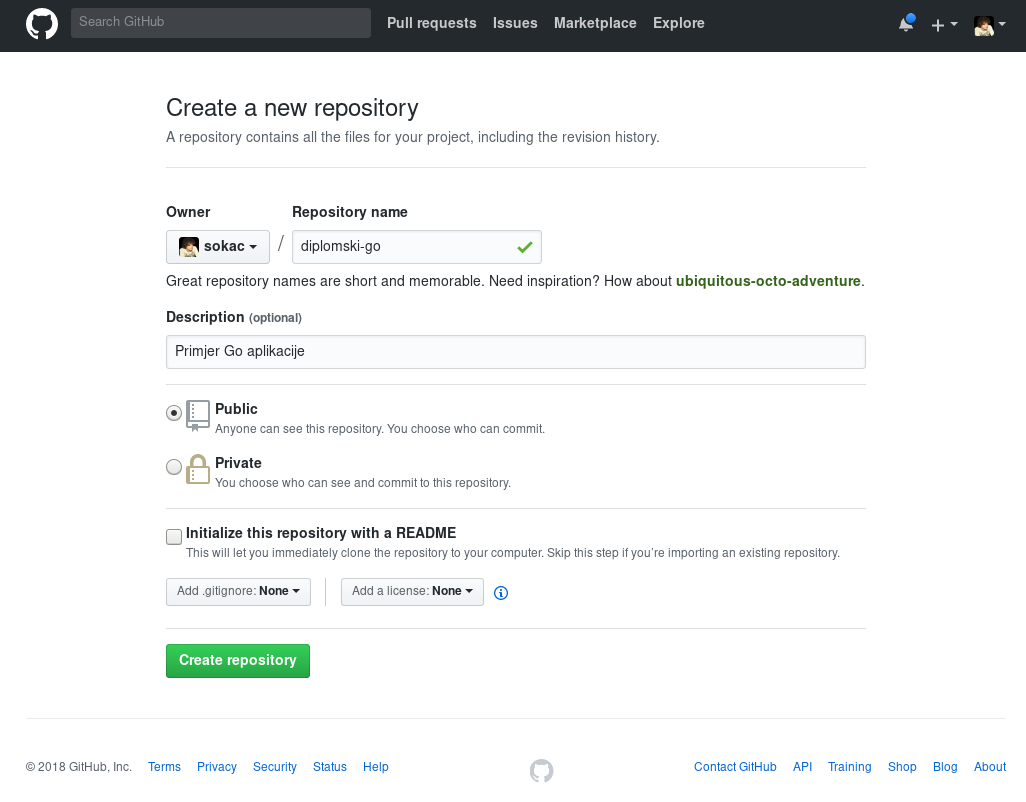
\includegraphics[width=0.7\linewidth]{img/02/gh.png}
    \caption{Registracija Git projekta na github.com}%
    \label{fig:02hgreg}
\end{figure}

Kada je napravljen projekt na GitHub-u, u lokalnu bazu registrira se udaljen Git poslužitelj pomoću
\textit{git-remote} operacije te se lokalna baza može poslati na udaljeno pomoću operacije
\textit{git-push}. Važno je zapamtiti da operacija \textit{git-commit} ne šalje izmjene na udaljeno
računalo, nego isključivo \textit{git-push}.  Operacija \textit{git-push} šalje samo razliku između
lokalnih predanih datoteka te udaljenih datoteka.  Primjer dodavanja udaljenog servera i slanje
izmjena dan je programskim kodom~\ref{02remote}

\lstset{caption={Dodavanje poslužitelja i slanje izmjena}, label=02remote}
\begin{lstlisting}[float=h]
git remote add origin git@github.com:sokac/diplomski-go.git
git push -u origin master
\end{lstlisting}

\subsection{Git grananje}
Većina VSC sustava podržava neku vrstu grananja. Grananje omogućuje korisniku da izađe iz glavne
grane razvoja, često nazvanu \textit{master}, te nastavi razvoj u potpuno drugoj grani. Korisnik u
bilo kojem trenutku može izabrati u kojoj grani želi biti. Također, korisnik može spojiti dvije
grane u bilo kojem trenutku.

Git ima prednost nad drugim VSC sustavima jer su stvaranje i mijenjanje grana izuzetno brze
operacije. Samim time, Git potiče na često korištenje grana. Kreiranje grane obavlja se operacijom
\textit{git-branch}, koja kreira novu granu. Takva grana ima iste datoteke kao i grana prije nego
što je operacija kreiranja grane bila pozvana. Operacija \textit{git-checkout} koristi se za
prebacivanje u drugu granu. Trenutna grana zapisana je u specijalnoj referenci koja se zove
\textit{HEAD}. Na slici~\ref{fig:02gitexample} prikazan je Git projekt s dvije grane,
\textit{master} i \textit{development}, gdje grana \textit{development} sadrži više predanih
izmjena. Prilikom pokretanja \textit{git checkout master}, \textit{HEAD} pokazivač se pomiče na
\textit{master} granu te se datoteke mijenjaju na sadržaj u tom trenutku, kao što je prikazano na
slici~\ref{fig:02gitexample2}. Ukoliko korisnik preda izmjene unutar grane \textit{master}, tada
dolazi do razdvajanja grana, jer grana \textit{master} ima datoteke koje ne postoje u povijesti
grane \textit{development} i obrnuto. Git operacija \textit{git-merge} omogućava spajanje grana i u
takvom slučaju.

\begin{figure}[h]
    \centering
    \begin{tikzpicture}[
        scale=1.0,
        node distance=3mm,
        text width=3.5cm,
        text centered,
        box/.style={
            minimum height=6mm,
            rectangle,
            rounded corners,
            draw=black,
            very thick,
            text centered,
            fill=yellow!10
        },
        head/.style={
            fill=orange!40
        },
        version/.style={
            fill=blue!10
        },
    ]
        \node [box, version] (c1version1) {Verzija 1};
        \node [box, version, right=of c1version1] (c1version2) {Verzija 2};
        \node [box, version, right=of c1version2] (c1version3) {Verzija 3};
        \node [box, above=of c1version2] (master) {master};
        \node [box, below=of c1version3] (development) {development};
        \node [box, head, below=of development] (head) {HEAD};
        \draw [<-] (c1version1) -- (c1version2);
        \draw [<-] (c1version2) -- (c1version3);
        \draw [->] (development) -- (c1version3);
        \draw [->] (master) -- (c1version2);
        \draw [->] (head) -- (development);

    \end{tikzpicture}

    \caption{Primjer Git grana}%
    \label{fig:02gitexample}
\end{figure}

\begin{figure}[h]
    \centering
    \begin{tikzpicture}[
        scale=1.0,
        node distance=3mm,
        text width=3.5cm,
        text centered,
        box/.style={
            minimum height=6mm,
            rectangle,
            rounded corners,
            draw=black,
            very thick,
            text centered,
            fill=yellow!10
        },
        head/.style={
            fill=orange!40
        },
        version/.style={
            fill=blue!10
        },
    ]
        \node [box, version] (c1version1) {Verzija 1};
        \node [box, version, right=of c1version1] (c1version2) {Verzija 2};
        \node [box, version, right=of c1version2] (c1version3) {Verzija 3};
        \node [box, above=of c1version2] (master) {master};
        \node [box, below=of c1version3] (development) {development};
        \node [box, head, above=of master] (head) {HEAD};
        \draw [<-] (c1version1) -- (c1version2);
        \draw [<-] (c1version2) -- (c1version3);
        \draw [->] (development) -- (c1version3);
        \draw [->] (master) -- (c1version2);
        \draw [->] (head) -- (master);

    \end{tikzpicture}

    \caption{Primjer pomicanja Git grane}%
    \label{fig:02gitexample2}
\end{figure}

Osim standardnih operacija, Github servis nudi uslugu pregleda koda (\textit{engl. code review}).
Inženjeri mogu međusobno pregledavati kod prije nego što se spoji s glavnom granom. Također, moguće
je koristiti i integracijske testove kako bi se osiguralo da novi kod ispravno funkcionira.

\section{Jenkins}
Timovi koji koriste stare metode, kao što su Grantt dijagrame i model vodopada (\textit{engl.
waterfall model}), moraju odvojiti poveći dio vremena za fazu integracije. U toj fazi razvoja
računalne podrške, inženjeri i timovi spajaju dijelove koda na kojima su radili mjesecima.  Prilikom
spajanja dijelova koda, često dolazi do sukoba datoteka i programskih sučelja koji inženjeri ručno
moraju riješiti. Taj proces zna potrajati tjednima kako bi se suboki riješili i program ponovno
testirao. U takvom sustavu, faza integracija izuzetno je stresna za inženjere i voditelje timove. Ta
faza često odgađa objavljivanje nove verzije aplikacije, a samim time i gubitak povjerenja krajnjih
korisnika. Iz tih razloga, nastala je potreba za kontinuiranom integracijom.

Kontinuirana integracija (CI, \textit{engl.~Continuous Integration}) je način razvoja aplikacije
gdje se radne verzije programa spajaju s glavnom verzijom barem jednom
dnevno~\citep{fowler2006continuous}.  Ekstremnija verzija takvog načina razvoja nazvana je ekstremno
programiranje (XP, \textit{engl.~Extreme Programming}), gdje se radna verzija spaja u glavnu verziju
barem jednom u dva do tri sata~\citep{beck1999embracing}. Kako bi to bilo moguće potrebna je dobra
infrastruktura koja omogućava brzo otkrivanje grešaka prilikom razvoja. Također, pomaže prilikom
dijagnostike te omogućava brzu izgradnju aplikacije. Svaki profesionalni razvojni tim treba
koristiti takav sustav kako bi bio što učinkovitiji i konkurentniji.

Pojednostavljeno, sustav kontinuirane integracije nadgleda sve promjene nad sustav kontrole verzija.
Kada je promjena očitana, sustav pokreće proces testiranja jedinica i izgradnje aplikacije
(\textit{engl. compile}). U slučaju greške, sustav obavještava inženjera o pogrešci kako bi se mogla
ispraviti što prije. Osim toga, sustav mora biti u mogućnosti proizvesti izvješća o kvaliteti koda,
kao što je pokrivenosti testiranja jedinice, razne statistike poput vrijeme izgradnje, učestalost
grešaka.

Ukoliko je sustav kontinuirane integracije pouzdan, može se automatizirati i sustav objavljivanja
aplikacija. Ukoliko se takva aplikacija automatski objavljuje i dostavlja krajnjim korisnicima, radi
se o sustavu za kontinuirani razvoj i objavu aplikacija (\textit{engl.~Continuous Deployment}). Kod
takvog sustava iznimno je bitno da je proces nadogradnje aplikacije jednostavan, a poželjno i
skriven, od krajnjeg korisnika. Stoga se najčešće primjenjuje na mrežnim aplikacijama, kao što su
internet aplikacije i stranice.

Jenkins, izvorno nazvan Hudson, je alat za kontinuiranu integraciju otvorenog koda napisan u
programskom jeziku Java. Postao je iznimno popularan zbog jednostavnosti korištenja, jednostavnog
grafičkog sučelja, mogućnost proširenja preko dodataka (\textit{engl. plugins}) te mnogih drugih
značajki. Uvođenje Jenkins alata može se uvesti postepeno u firmama koji nemaju nikakav
sustav~\citep{smart2011jenkins}. Prvo je potrebno uvesti sustav koji će na dnevnoj bazi izgrađivati
aplikaciju. Druga faza je uvođenje automatskog testiranja prije izgrađivanja aplikacije, također na
dnevnoj razini. Sljedeća faza je uvođenje metrika vezano za kvalitetu koda (pokrivenosti jedinica,
brzina testova i izgradnje) te automatska izgradnja dokumentacije. Četvrta faza je dodatno
testiranje, kao što je testiranje funkcionalnosti. Takvo testiranje odvija se nakon što je
aplikacija izgrađena. Peta faza je gdje se aplikacija koja je prošla dodatno testiranje automatski
objavljuje. Takvu aplikaciju mogu koristiti osobe koje nisu inženjeri, kao što su timovi za
testiranje kvalitete. Zadnja faza sustava je kontinuirano objavljivanje aplikacije krajnjim
korisnicima.

Jenkins se sastoji od Jenkins poslova (\textit{engl. Jenkins Jobs}), Jenkins građe (\textit{engl.
Jenkins build}), parametara, Jenkins linije (\textit{engl. Jenkins Pipeline}) i dodataka.

\subsection{Jenkins arhitektura}
Jenkins posao je skup pravila prema kojem se izgrađuje aplikacija. Sastoji se od naziva posla,
opisa, definira parametre potrebne za pokretanje izgradnje aplikacije, instrukcija kako se izgrađuje
aplikacija te listu akcija nakon što je posao završen~\citep{pathania2016learning}. Jenkins posao ne
ovisi o programskom jeziku aplikacije koja se izgrađuje, niti o VCS. Posao se može programirati, ali
i izgraditi koristeći grafičko web sučelje. Primjer izgradnje posla preko web sučelja prikazan je
slikom~\ref{fig:02jenkinsjob}

\begin{figure}
    \centering
    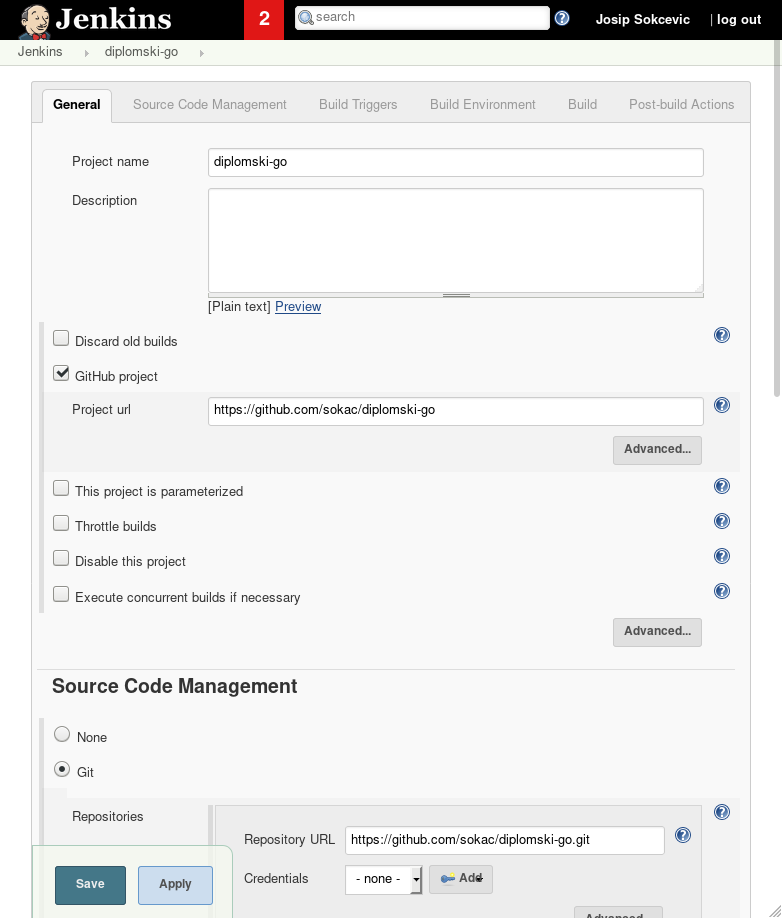
\includegraphics[width=0.5\textwidth]{img/02/jenkins_job.png}
    \caption{Izgradnja Jenkins posla}%
    \label{fig:02jenkinsjob}
\end{figure}

Jenkins parametri se najčešće koriste za Jenkins poslove. Jenkins podržava velik broj tipova
parametara, kao što su riječi, brojevi, izbornici, jedno-bitni podaci (da/ne odgovor). Parametri se
mogu automatski predavati poslu ili ručno. Primjer automatskog predavanja parametara je kada jedan
Jenkins posao pokreće drugi te predaje informacije o prethodnom izvršavanju. Primjer ručnog
predavanja parametara je kada korisnik odabere verziju koju želi pokrenuti.

Većina Jenkins poslova sadrže barem jednu Jenkins građu. Jenkins građa je jedinica posla koja se
izvršava kada se posao izvršava. Može biti jednostavna Linux Bash ili Windows batch naredba, a preko
dodataka može izvršavati i kompleksne stvari kao što su Python skripte, preuzimanje Android
dodataka. Jedan Jenkins posao može imati više Jenkins građi.

Jenkins linija omogućuje umrežavanje više Jenkins poslova. Linija može pokrenuti Jenkins poslove
sekvencijalno ili paralelno te može sadržavati logiku. Na primjer, Jenkins linija može odlučiti da
se linija prekida ukoliko jedan od paralelnih poslova bude neuspješan. Pomoću akcija nakon građe
(\textit{engl. Post-Build}), korisnici mogu biti obaviješteni o rezultatima građe.

Jedna od velik prednosti Jenkins alata jest upravo u dodacima. Dodaci mogu mijenjati vizualno web
sučelje, mijenjati način povezivanja Jenkins gazde s Jenkins slugom, dodati podršku za nove
programske jezike i VSC. U službenom Jenkins repositoriju registrirano je preko tisuću različitih
dodataka~\citep{JenkisPlugins}.

\section{Cypress}
Cypress je alat za integracijsko i \textit{end-to-end} testiranje web stranica i aplikacija. Za
razliku od sličnih alata, kao što je Selenium, pokretanje Cypressa je vrlo jednostavno, ima potpuni
pristup pregledniku koji vrši testiranje te pojednostavljeno programsko sučelje~\citep{Cypress}.

End-to-end testiranje web stranica služi kao simuliranje stvarnih korisnika. Na primjer, ukoliko
jedan od elemenata nije prikazan unutar internet preglednika jedino \textit{end-to-end} testiranje
može otkriti takvu grešku. No, \textit{end-to-end} testiranje je vremenski zahtjevno za pisanje, a
pogotovo za održavanje. Bilo kakva vizualna promjena na aplikaciji zahtjeva promjenu
\textit{end-to-end} testova, a promjena u funkcionalnosti zahtjeva potpuno nove testove. Stoga je
preporuka Googleovih inženjera da je 70\% testova jedinice, 20\% integracijski testova, a svega 10\%
\textit{end-to-end} testovi~\citep{google-2015}.

Otvaranje Cypress alata na lokalnom računalu odvija se preko naredbe $cypress~start$ koja otvara
program za pokretanje testova, kao što je prikazanom slikom~\ref{fig:02cypress}. Preko aplikacije
korisnik može pokrenuti testove te vidjeti rezultate. Cypress alat prati izmjene konfiguracije na
tvrdom disku te ih automatski učitava ako dođe do izmjene.

\begin{figure}[h]
    \centering
    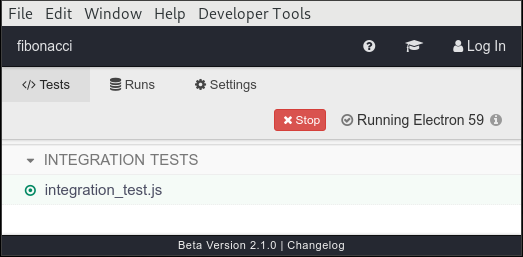
\includegraphics[width=0.8\textwidth]{img/02/cypress.png}
    \caption{Cypress aplikacija}%
    \label{fig:02cypress}
\end{figure}

Cypress testovi se mogu pokrenuti i preko komandne linije što je poželjno prilikom pokretanja na
Jenkins poslužitelju. Pokretanje testa izvršava se naredbom $cypress~run$. Cypress zatim pokreće
preglednik u takozvanom \textit{headless} načinu rada, to jest bez grafičkog sučelja. Nakon
završetka rada, Cypress izlazni rezultat sadrži informaciju o uspješnosti testa. Cypress može
spremiti sve rezultate u junit XML formatu. Primjer uspješnog rezultata dan je
kodom~\ref{02cypressxml}.

\lstset{caption={junit XML rezultat}, label=02cypressxml}
\begin{lstlisting}[float=h]
<?xml version="1.0" encoding="UTF-8"?>
<testsuites name="Mocha Tests" time="1.321" tests="2" failures="0">
  <testsuite name="Root Suite" timestamp="2018-03-19T03:14:07" tests="0" failures="0" time="0">
  </testsuite>
  <testsuite name="Fibonacci test" timestamp="2018-03-19T03:14:07" tests="2" failures="0" time="1.321">
    <testcase name="Fibonacci test Ispravna forma" time="0.744" classname="Ispravna forma">
    </testcase>
    <testcase name="Fibonacci test Neispravna forma" time="0.577" classname="Neispravna forma">
    </testcase>
  </testsuite>
</testsuites>
\end{lstlisting}

\section{Docker}
Docker je projekt otvorenog koda napisan u Go programskom jeziku koji pojednostavljuje objavljivanje
programa tako što koristi programske kontejnere (\textit{engl. Software Containers}). Docker slika
pakira program unutar cjelokupnog datotečnog sustava koji ima sve potrebne komponente kako bi se
takav program mogao izvoditi - od dinamičkih modula, biblioteka, sve do programskog sučelja
operativnoga sustava. Stoga, Docker garantira da će izvršavanje takvog sustava bit uvijek jednako,
neovisno o računalo na kojem se izvodi.

Konceptno, Docker je sličan virtualizaciji, kao što je VMWare i VirtualBox. No, za razliku od njih,
Docker ima prednosti u tome što je brži i koristi manje resursa~\citep{leszko2017continuous}. Na
slici~\ref{fig:02vm} prikazana je arhitektura kod tipične virtualizacije, dok je na
slici~\ref{fig:02docker} prikazana  Docker arhitektura.

\begin{figure}[h]
    \centering
    \begin{tikzpicture}[
        scale=1.0,
        node distance=1mm,
        text width=3.5cm,
        text centered,
        box/.style={
            minimum height=8mm,
            rectangle,
            draw=black,
            very thick,
            text centered,
        },
        box1/.style={
            fill=yellow!10,
        },
        box2/.style={
            fill=blue!10,
        },
        box3/.style={
            fill=green!10,
        },
        os/.style={
            minimum height=16mm,
        },
        big/.style={
            fill=orange!40,
            text width = 11.8cm,
        },
    ]
        \node [box, big] (server) {Poslužitelj};
        \node [box, big, above=of server] (os) {Operativni sustav};
        \node [box, big, above=of os] (vmm) {VMM - Virtual Machine Monitor};

        \node [box, box2, os, above=3mm of vmm] (g2os) {OS gosta};
        \node [box, box2, above=of g2os] (g2bib) {Biblioteke};
        \node [box, box2, above=of g2bib] (g2app) {Aplikacija 2};

        \node [box, box1, os, left=3mm of g2os] (g1os) {OS gosta};
        \node [box, box1, above=of g1os] (g1bib) {Biblioteke};
        \node [box, box1, above=of g1bib] (g1app) {Aplikacija 1};

        \node [box, box3, os, right=3mm of g2os] (g3os) {OS gosta};
        \node [box, box3, above=of g3os] (g3bib) {Biblioteke};
        \node [box, box3, above=of g3bib] (g3app) {Aplikacija 3};
    \end{tikzpicture}

    \caption{Arhitektura virtualizacije}%
    \label{fig:02vm}
\end{figure}

\begin{figure}[h]
    \centering
    \begin{tikzpicture}[
        scale=1.0,
        node distance=1mm,
        text width=3.5cm,
        text centered,
        box/.style={
            minimum height=8mm,
            rectangle,
            draw=black,
            very thick,
            text centered,
        },
        box1/.style={
            fill=yellow!10,
        },
        box2/.style={
            fill=blue!10,
        },
        box3/.style={
            fill=green!10,
        },
        big/.style={
            fill=orange!40,
            text width = 11.8cm,
        },
    ]
        \node [box, big] (server) {Poslužitelj};
        \node [box, big, above=of server] (os) {Operativni sustav};
        \node [box, big, above=of os] (docker) {Docker engine};

        \node [box, box2, above=3mm of docker] (g2bib) {Biblioteke};
        \node [box, box2, above=of g2bib] (g2app) {Aplikacija 2};

        \node [box, box1, left=3mm of g2bib] (g1bib) {Biblioteke};
        \node [box, box1, above=of g1bib] (g1app) {Aplikacija 1};

        \node [box, box3, right=3mm of g2bib] (g3bib) {Biblioteke};
        \node [box, box3, above=of g3bib] (g3app) {Aplikacija 3};
    \end{tikzpicture}

    \caption{Docker arhitektura}%
    \label{fig:02docker}
\end{figure}

Docker slika (\textit{engl. Docker Image}) je preslika datotečnog sustava koja se sastoji od niza
Docker slojeva (\textit{engl. Docker layers}). Slojevi predstavljaju promjene u datotečnom sustavu
naspram prijašnjeg sloja. Docker kontejner koristi Docker sliku te pokreće određenu aplikaciju koja
se već nalazi unutar Docker slike. Promjene unutar Docker kontejnera, kao što je zapis novih
datoteka, ne mijenjaju Docker sliku koja je korištena za pokretanje tog kontejnera. Kada se Docker
kontejner zaustavi i obriše, svi podaci su također obrisani.

Docker slike mogu se spremiti u Docker repositorij koji može biti privatni ili javni. Jedan od
najčešće korištenih je službeni repositorij firme koja stoji iza Docker-a - Docker, Inc, a koji se
nalazi na Web stranici \textit{https://hub.docker.com}.

\subsection{Docker operacije}

Izgradnja Docker slike pokreće se pomoću naredbe $docker~build$. Ta naredba učitava datoteku
\textit{Dockerfile} u zadanom direktoriju. \textit{Dockerfile} je tekstualni dokument koji sadrži
instalacijske instrukcije potrebne za izgradnju Docker slike~\citep{kacamarga2015lightweight}.
Na primjeru danim kodom~\ref{02dockerfile} prikazana je instalacija Jenkins alata.

\lstset{caption={Jenkins Dockerfile}, label=02dockerfile}
\begin{lstlisting}[float=h]
FROM openjdk:8-jdk-alpine

RUN addgroup -g 1000 jenkins
RUN adduser -u 1000 -G jenkins jenkins

RUN curl -fsSL \
    https://repo.jenkins-ci.org/public/org/jenkins-ci/main/jenkins-war/2.117/jenkins-war-2.117.war \
    -o /usr/share/jenkins/jenkins.war

USER jenkins

ENTRYPOINT ["java", "-jar", "/usr/share/jenkins/jenkins.war"]
\end{lstlisting}

U danom primjeru korištene su četiri naredbe. Naredbna $FROM$ definira Docker sliku na kojoj će se
nova slika temeljiti. Na primjeru, temelji se na \textit{openjdk} slici pod oznakom
\textit{8-jdk-alpine}. Naredba $RUN$ pokreće program koji je definiran iza te naredbne. U danom
primjeru, pokrenuta je komanda $addgroup$ koja stvara Jenkins groupu, komada $adduser$ koja stvara
Jenkins korisnika te $curl$ koja dohvaća Jenkins alat s udaljenog računala.
Naredba $USER$ definira pod kojim korisnikom se pokreće Docker kontejner. U danom primjeru, to je
korisnik "jenkins". Zadnja korištena naredba $ENTRYPOINT$ koja definira koji će se program pokrenuti
unutar Docker kontejnera, a u danom primjer je $java -jar /usr/share/jenkins/jenkins.war$.

Nakon što je Docker slika izgrađena, korisnik može pokrenuti Docker kontejner koristeći
novoizgrađenu sliku pomoću naredbe $docker~run$. Prilikom pokretanja takve naredbe, korisnik može
podesiti mrežne postakve, montirati direktorije, ograničiti procesorske, diskovne i memorijske
resurse, izmjeniti sigurnosne postavke te mnoge druge parametre.

Jedan od najčešće korištenih parametera za mrežne aplikacije jeste parametar $-p$. Prilikom
pokretanja Docker kontejnera, mreža je podešena u tzv.~\textit{bridge} načinu rada te samim time
pristup Docker kontejneru nije moguć u lokalnoj mreži. Parametar $-p$ naređuje Docker sustavu
da objavi mrežni port unutar kontejnera na glavnom računalu. Na primjer, parametar $-p 8080:80$
preusmjerava mrežne zahtjeve porta 8080 na glavnom računalu prema mrežnom portu 80 unutar Docker
kontejnera. Promjena mrežnog načina rada moguća je preko parametra $--network$.

Svi podaci koji su spremljeni unutar kontejnera su trajno obrisani pri brisanju istoga. Montiranje
direktorija koristi se ukoliko aplikacija sprema bitne podatke na tvrdi disk te nije dopušteno
brisanje. Svi zapisi na montirani direktorij spremaju se na tvrdi disk glavnog računala, a Docker
kontejner ima puni pristup njima. Na primjer, parametar $-v /glavno/racunalo:/data$ montira
direktorij glavnog računala pod nazivom $/glavno/racunalo$ na direktorij Docker kontejnera pod
nazivom $/data$. Kada Docker kontejner napravi izmjenu unutar $/data$ direktorija, takva izmjena
biti će automatski dostupna unutar glavnom računala pod direktorijom $/glavno/racunalo$.

Zaustavljanje pokrenutog Docker kontejnera izvršava se pomoću naredbe $docker~stop$ koja prihvaća
listu Docker kontejnera koje se želi ugasiti. Docker servis prvo šalje \textit{SIGTERM} signal
aplikaciji. Ukoliko aplikacija nije zaustavljane unutar perioda milosti (\textit{engl. grace
period}), tada Docker šalje \textit{SIGKILL} signal.

Zaustavljeni Docker kontejner može se ponovno pokrenuti naredbom $docker~start$. Naredbom
$docker~rm$ briše se kontejner zajedno sa svim podacima spremljenim unutar kontejnera.

\section{Nginx}
Nginx je web poslužitelj otvorenog koda napisan u C programskom kodu koji se često koristi kao
balansiranje opterećenja (\textit{engl. Load Balancer}) i obrnuti posrednik (\textit{engl. reverse
proxy}). Nastao je s ciljem da ima bolje performanse nego Apache web poslužitelj. Prema analizi iz
2017. godine, Nginx i dalje ima bolje performanse nego Apache~\citep{nguyen2017comparative}.
Firma Netcraft, koja se bavi istraživanjem web stranica i servisa, obavlja istraživanje svakih
mjesec dana. U veljači 2018. godine svaka četvrta internet stranica bila je posluživanja preko Nginx
poslužitelja~\citep{Netcraft2018}.

Nginx se sastoji od glavnog procesa koji raspodjeljuje posao radnicima. Radnik je proces koji prima
naredbe od glavnog procesa te je baziran na asinkorniziranom principu~\citep{reese2008nginx} te se
oslanja na Linux sistemske pozive $epoll/select/poll$. Stoga, radnik poslužuje više zahtjeva
odjednom s izuzetno malo dodatnih resursa. Zbog toga se Nginx često koristi kao balanser
opterećenja.

Balansiranje opterećenja je potreban ukoliko jedan poslužitelj aplikacije nema dovoljno resursa kako
bi poslužio sve klijente~\citep{soni2016load}. Nginx podržava pet algoritama balansiranja te je na
korisniku da utvrdi koji je najbolji za aplikaciju. Prilikom korištenja balancera opterećenja, Nginx
služi kao obrnuti posrednik. Klijenti se spajaju na Nginx koji zatim odlučuje, ovisno o definiranim
pravilima, gdje će proslijediti takav zahtjev. Nginx ima mogućnost dodati i uređivati određene
informacije na takav zahjev. Nakon primitka odgovora, Nginx također ima mogućost promjene
informacija. Takav obrađeni odgovor se zatim šalje klijentu.

\subsection{Nginx konfiguracija}
Pri pokretanju Nginx poslužitelja potrebno je zadati konfiguracijsku datoteku. Konfiguracijska
datoteka sadrži informacije o mrežnim protokolima i mrežnim portovima. Ukoliko se Nginx koristi kao
balanser opterećenja ili obrnuti posrednik, korisnik tada mora definirati gdje će se zahtjevi
proslijediti. Primjer minimalne Nginx konfiguracije prikazan je kodom~\ref{02nginxconfig}

\lstset{caption={Nginx konfiguracija}, label=02nginxconfig}
\begin{lstlisting}[float=h]
worker_processes  1;

events {
    worker_connections  1024;
}

http {
    server {
        listen       80;
        server_name  localhost;

        location / {
            proxy_pass https://www.ferit.unios.hr;
        }
    }
}
\end{lstlisting}

Parametar $worker\_process$ je broj radnih procesa kojih će Nginx poslužitelj pokrenuti. Svaki
proces izvršava se samo na jednoj procesorskoj jezgri pa se preporuča vrijednost jednakoj broju
dostupnih procesorskij jezgri. Blok $events$ definira kako će se obraditi korisnički zahtjevi.
Unutar toga bloka, $worker\_connections$ definira maksimalni broj paralelnih zahtjeva po radniku.

Unutar $http$ bloka nalazi se $server$ blok koji naređuje Nginx da prihvaća zahtjeve na određenom
mrežnom portu. U danom primjeru, to je port 80. $server\_name$ je naziv domene za koju će zahtjev
biti obrađen. Domena je dostupna preko $HTTP$ zaglavlja naziva $Host$, definiranog u RFC
2616~\citep{fielding1999hypertext}. Nadalje, $location$ blok definira kako će se svi zahtjevi
obraditi. Pomoću naredbe $proxy\_pass$, moguće je preusmjeriti zahjev na proizvoljni poslužitelj. Na
primjeru danom kodom~\ref{02nginxconfig}, svi $HTTP$ zahtjevi prosljeđeni su na $www.ferit.unios.hr$
server.

Nginx proces učitava konfiguracijsku datoteku prilikom pokretanja. Prilikom izmjene konfiguracijske
datoteke potrebno je ponovno učitati konfiguracijsku datoteku. To se može pokretanjem nginx procesa
s parametrom $-s reload$, ponovnim pokretanjem servisa pomoću $systemd reload nginx$ ili slanjem
Unix signala $SIGHUP$. Novu konfiguraciju moguće je učitati pomoću gašenja i ponovnog paljena Nginx
servisa, no s takvom metodom aplikacije će nakratko biti nedostupna.

\section{Go programski jezik}
Go je programski jezik otvorenog koda razvijen od firme Google. Projekt je nastao 2007. godine, a
prva verzija javno je objavljena 2009. godine. Go jezik inspiriran je C programskim jezikom te manje
poznatim Alef i Oberon-2 jezicima~\citep{donovan2015go}.

Od C programskog jezika Go je naslijedio sintaksu, način kontrole toka programa, osnovne tipove
podataka, pokazivače te brzo izvođenje programa i neovisnost o trenutnom operativnom sustavu.
Od Oberon-2 naslijeđena je sintaksa za programske pakete, uključivanje istih te deklaraciju metoda
i funkcija. Od jezika Alef naslijeđeni su kanali kao način komunikacije između procesa bez potrebe
za dijeljenom memorijom.

Primjer jednostavne \textit{Hello, World} aplikacije dan je kodom~\ref{02goexample}.

\lstset{caption={Go primjer}, label=02goexample}
\begin{lstlisting}[float=h]
package main

import "fmt"

func main() {
    fmt.Println("Hello, World")
}
\end{lstlisting}

Kako je Go prevođeni jezik, potrebno je prevesti Go kod u računalni program. Naredba $go build$
pokreće Go prevoditelj i, ukoliko je prevođenje uspješno, stvara binarnu datoteku koja se može
pokrenuti.

Go je organiziran u pakete (\textit{engl. packages}), što bi u drugim programskim jezicima bile
biblioteke ili moduli. Go paket se sastoji od jednog ili više Go izvornih datoteka unutar istog
direktorija. U danom primjeru, naziv paketa je $main$.

Go standardna biblioteka sadrži preko 100 paketa za uobičajne zadaće kao što su ulazi/izlazi,
manipuliranje teksta, sortiranje, kriptografke funkcije. Paket $fmt$ korišten u primjeru sadrži
funkcije za obradu ulaza te ispis formatiranog izlaza. Funkcija $Println$ ispisuje jednu ili više
vrijednosti odvojenih zarezom na standardni izlaz s novim rednom na kraju ispisa.

Go prevoditelj je strog oko pravila pisanja izvorne datoteke. Program $gofmt$ koristi se za
preoblikovanje izvorne datoteke. Na primjer, ukoliko je korišten razmak umjesto tabulatora, $gofmt$
će zamjeniti razmake sa tabulatorom.


